% MSC2020: 11J70 (continued fractions), 11G05 (elliptic curves over global fields), 11Y65 (continued fraction calculations), 39A06 (linear difference equations), 41A21 (Padé approximation)
% Keywords: polynomial continued fractions, Birkhoff-Trjitzinsky, j-invariant, CM elliptic curves, WKB asymptotics, AEAL methodology
\documentclass[11pt]{amsart}
\usepackage[T1]{fontenc}
\usepackage{amsmath,amsthm,amssymb,mathrsfs}
\usepackage[margin=1in]{geometry}
\usepackage{graphicx}
\usepackage[hidelinks]{hyperref}
\hypersetup{pdftitle={A j-invariant-correlated cubic finer-split in polynomial continued-fraction asymptotics},pdfauthor={papanokechi}}
\setlength{\textfloatsep}{8pt plus 2pt minus 2pt}
\setlength{\abovecaptionskip}{4pt}
\setlength{\belowcaptionskip}{0pt}

\theoremstyle{plain}
\newtheorem{theorem}{Theorem}
\newtheorem{conjecture}{Conjecture}
\theoremstyle{definition}
\newtheorem{definition}{Definition}
\newtheorem{remark}{Remark}
\newtheorem{problem}{Open problem}

\newcommand{\claim}[1]{\textup{\textsf{#1}}}
\newcommand{\PCF}{A_{\mathrm{PCF}}}

\title[A j-invariant-correlated cubic finer-split]{A j-invariant-correlated cubic finer-split in polynomial continued-fraction asymptotics}
\author{papanokechi}
\date{2026-05-01}

\begin{document}

\begin{abstract}
For a polynomial continued fraction generated by an integer polynomial \(b\) of degree \(d\), the convergent-error sequence has a WKB asymptotic with leading exponent \(\PCF(b)\), whose sharp PCF-2 Conjecture B4 predicts \(\PCF=2d\).  We report a degree-3 finer split: R1.1 found \(\rho(\log(|j(E_b)|+1),A_{\rm fit}-6)=-0.691\), and R1.3 reproduced it at deep precision with \(\rho=-0.5683\), Bonferroni \(p=5.0\times10^{-5}\), on 50 cubic families.  The four equianharmonic CM families in the \(j=0\) cell, with Weierstrass pattern \((1,-3,3,*)\), hit \(A=6\) to \(\le 10^{-3}\).  The sharp statement does not extend to degree 4: R13-C shows a real shallow-\(N\) \(j=0\) shift, but R13-D deep-WKB gives fam32 \(\delta=-4.55\times10^{-4}\) and matched non-\(j=0\) fam01 \(\delta=-4.60\times10^{-4}\), a \(0.24\) pooled-stderr difference.  We therefore frame the phenomenon as cubic-modular, not as a cross-degree \(j\)-law; an Eisenstein/CM explanation is deferred to companion theory work.  Companion records: PCF-1 v1.3 DOI 10.5281/zenodo.19937196; PCF-2 v1.2 DOI 10.5281/zenodo.19951458; Channel Theory v1.2 DOI 10.5281/zenodo.19951331; SIARC umbrella DOI 10.5281/zenodo.19885550.
\end{abstract}
\maketitle



\section{Setup and verdict}

Let \(b(n)=a_d n^d+\cdots+a_0\in \mathbb Z[n]\) be primitive and irreducible.  The polynomial continued fraction
\[
L(b)=b(0)+\frac{1}{b(1)+\frac{1}{b(2)+\cdots}}
\]
has convergents \(L_N=P_N/Q_N\) obtained from the usual second-order recurrence.  The empirical PCF programme fits
\[
\log |L_N-L|=-\PCF(b)N\log N+\alpha N+\beta \log N+\gamma+o(1),
\]
and PCF-2's sharp B4 form predicts \(\PCF(b)=2d\) \cite{pcf2v12}.  This note studies only the residual finer split \(\delta_d(b)=A_{\rm fit}(b)-2d\).

The verdict is deliberately narrow.  At degree \(3\), \(E_b:y^2=b(x)\) is itself a nonsingular elliptic curve with its standard \(j\)-invariant; the observed signal is therefore a cubic-modular signal.  We do not conjecture cross-degree universality in the sharp/deep-WKB form.  Degree \(4\) still has a genus-one Jacobian and a \(j\)-invariant, but the R1.3 deep test rejects the analogous sharp rule.  Claim labels such as \claim{R11-3} and \claim{R13-D-4} refer to AEAL entries in the bridge data citations \cite{r11bridge,r13bridge}.

\section{The cubic finer split}

\begin{theorem}[Empirical degree-3 verification]
On the 50-family lex-window cubic catalogue, the \(j\)-invariant of \(E_b\) is a statistically significant predictor of \(\delta_3=A_{\rm fit}-6\), while the \(j=0\) CM cell sits at the sharp value \(A=6\) to \(\le 10^{-3}\).
\begin{enumerate}
\item R1.1 found \(\rho(\log(|j|+1),\delta_3)=-0.6906\), raw \(p=2.86\times10^{-8}\), Bonferroni \(p=4.0\times10^{-7}\) with \(K=14\) effective tests; the signal also passed the stricter \(K=20\) accounting (\claim{R11-3}).
\item R13-A reproduced the signal at dps\(=2000\), \(N\in[50,250]\), \(N_{\rm ref}=400\): \(\rho(\log(|j|+1),\delta^{\rm free}_{3})=-0.5683\), raw \(p=1.67\times10^{-5}\), Bonferroni \(p=5.01\times10^{-5}\) (\claim{R13-A-3}).
\item The four \(j=0\) families, equivalently the equianharmonic CM subcell with Weierstrass coefficient pattern \((1,-3,3,*)\), are the closed-form candidates for \(A=6\); R1.1 precision escalation placed the cell at \(\le 10^{-3}\) and R1.3 retains the same cell-level interpretation (\claim{R11-1}, \claim{R13-A-3}).
\end{enumerate}
\end{theorem}

\begin{figure}[t]
\centering
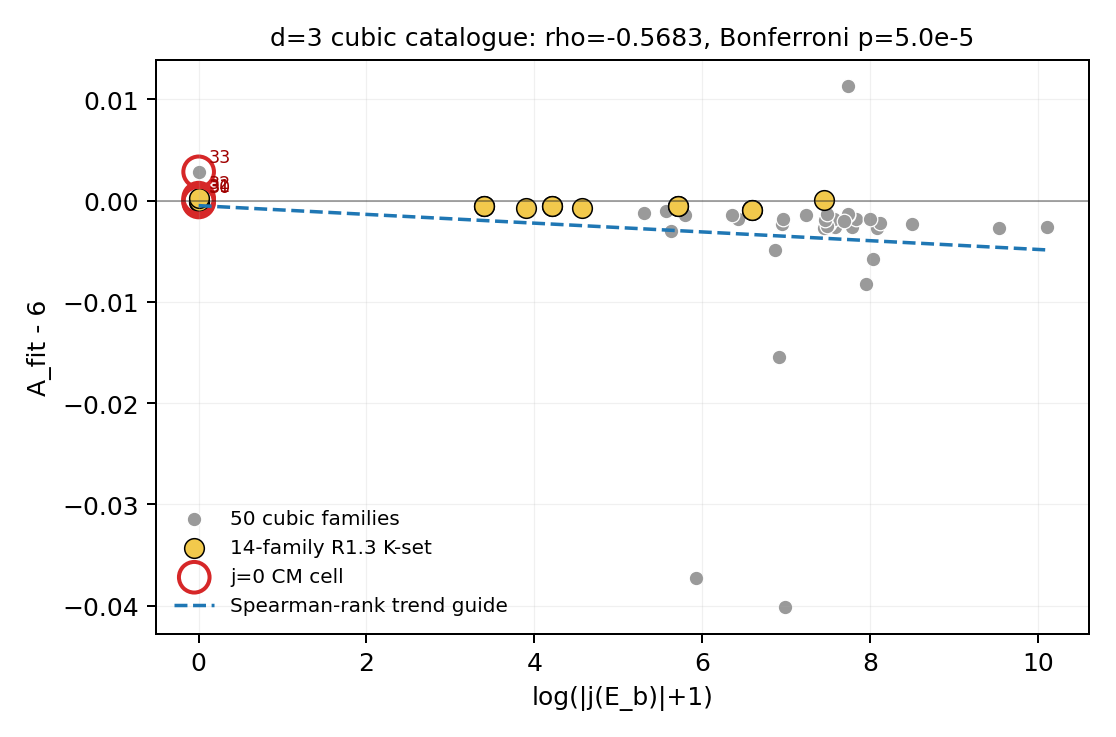
\includegraphics[width=0.72\linewidth]{j_scatter.png}
\caption{Cubic scatter of \(\log(|j(E_b)|+1)\) against \(A_{\rm fit}-6\) from R13-A.  Gray marks all 50 cubic families, gold marks the 14-family R1.3 diagnostic \(K\)-set generated by \texttt{make\_figure.py}, and red open circles mark the four \(j=0\) equianharmonic CM families.  The dashed line is a Spearman-rank trend guide for the negative association.  This plot is \(d=3\) only; a \(d=4\) analog is shown in a separate companion plot to be deferred to a longer paper.}
\label{fig:cubic-scatter}
\end{figure}

The figure is descriptive rather than a proof: the substantive thesis is not that the symbol \(j\) alone controls every PCF asymptotic, but that at \(d=3\) the PCF recurrence appears to see the modular structure of the elliptic curve \(E_b\).  The statistical statement is the Bonferroni-protected rank correlation; the cell statement is the special CM locus \(j=0\).

\section{Precision-stratified non-extension to degree 4}

The degree-4 analogue was tested explicitly in R1.3 and is not supported in sharp/deep-WKB form.  On the original Q1 quartic catalogue, R13-B found no rank signal: \(\rho(\log(|j|+1),\delta^{\rm free}_{4})=+0.0732\), Bonferroni \(p=1\) (\claim{R13-B-6}).  The catalogue contains only one \(j=0\) quartic, so R13-C then enumerated an extended \(j=0\) cell.  That shallow-\(N\) calculation found a real shift toward zero: after outlier removal, the \(j=0\) median was \(-2.493\times10^{-3}\), versus \(-3.727\times10^{-3}\) for the Q1 non-\(j=0\) cluster, with Mann--Whitney \(p=4.8\times10^{-4}\) unstratified and \(p=1.1\times10^{-6}\) after stratifying on coefficient sum (\claim{R13-C-12}, \claim{R13-E-25}).  This paragraph is part of the claim: the shallow effect is not hidden.

The referee-defense point is that R13-D then pushed the decisive comparator to deep WKB precision.  At dps\(=5000\), \(N_{\rm ref}=1000\), \(N\in[200,800]\), the unique Q1 \(j=0\) quartic family 32 gave
\[
\delta^{\rm deep}_{4}(\mathrm{fam32})=-4.5502\times10^{-4}\pm1.45\times10^{-5},
\]
while a matched non-\(j=0\) baseline, family 1, gave
\[
\delta^{\rm deep}_{4}(\mathrm{fam01})=-4.5993\times10^{-4}\pm1.47\times10^{-5}.
\]
The difference \(4.91\times10^{-6}\) is only \(0.24\) pooled standard errors (\claim{R13-D-1}, \claim{R13-D-3}, \claim{R13-D-4}, \claim{R13-E-24}).  Thus the R13-C shift is a precision-stratified shallow-\(N\) diagnostic, not a deep leading-exponent rule.  We explicitly disclaim a cross-degree statement of the form \(j=0\Rightarrow \PCF=2d\) or \(\rho(\log|j|,\delta_d)<0\) for all \(d\ge3\).

\section{Cubic-modular interpretation}

For cubics, the affine model \(E_b:y^2=b(x)\) is the elliptic curve whose \(j\)-invariant is measured.  The cell \(j(E_b)=0\) is the equianharmonic CM point with endomorphism ring \(\mathbb Z[\zeta_3]\).  A natural interpretation is that the leading Birkhoff--Trjitzinsky/WKB exponent for the cubic PCF recurrence is sensitive to the Eisenstein modular structure of \(E_b\), pinning the CM cell to the sharp value and inducing a monotone rank drift away from it.

This is still empirical.  The degree-4 failure shows that a genus-one Jacobian and a numerical \(j\)-invariant are not sufficient, by themselves, to force the leading exponent.  A proof would need to connect the recurrence's Newton polygon or channel-theory normal form to the Eisenstein CM specialization.  The companion PCF-1, PCF-2, Channel Theory, and SIARC records give the surrounding framework \cite{pcf1v13,pcf2v12,channelv12,siarcumbrella}.

\begin{problem}
Derive the degree-3 \(j=0\) value \(\PCF=6\) directly from the Birkhoff--Trjitzinsky expansion or an Eisenstein/CM normal form for \(E_b\).
\end{problem}

\begin{problem}
Explain the R13-C shallow-\(N\) quartic shift as a sub-leading WKB term, and prove why it vanishes from the deep leading exponent.
\end{problem}

\section*{Reproducibility and AEAL note}

The numerical source files are the R1.1 and R1.3 bridge directories \cite{r11bridge,r13bridge}.  R1.3 scripts include \texttt{r1\_3\_residualization.py}, \texttt{r1\_3\_extended\_enumeration.py}, \texttt{r1\_3\_family32\_deep.py}, and \texttt{r1\_3\_phase\_E\_final.py}; the concatenated R1.3 audit log contains 26 claims.\footnote{Empirical claims in this note are documented as AEAL (Asynchronous Empirical Audit Log) claims with full statistical evidence at the bridge URLs in the bibliography. Each claim\_id can be queried for its full provenance.}  The DOI records cited here were checked through \texttt{doi.org} before packaging.

\clearpage
\bibliographystyle{plain}
\bibliography{standalone_note}

\end{document}






